\setcounter{secnumdepth}{4}
\chapter{Produktspezifikationen}
Dieses Kapitel behandelt die Planung und Spezifikation des Projekts.
Weiteres wird die verwendete Technologieauswahl begründet und mit Alternativlösungen verglichen.

\section{Anforderungen und Spezifikationen}
Hier steht der allgemeine Text für die Anforderungen und Spezifikationen

\subsection{Use Cases}
Hier steht der allgemeine Text für die Use Cases

\section{Design}
Hier steht der allgemeine Text für das Design

\subsection{Abläufe}
\begin{figure}[h]
    \centering
    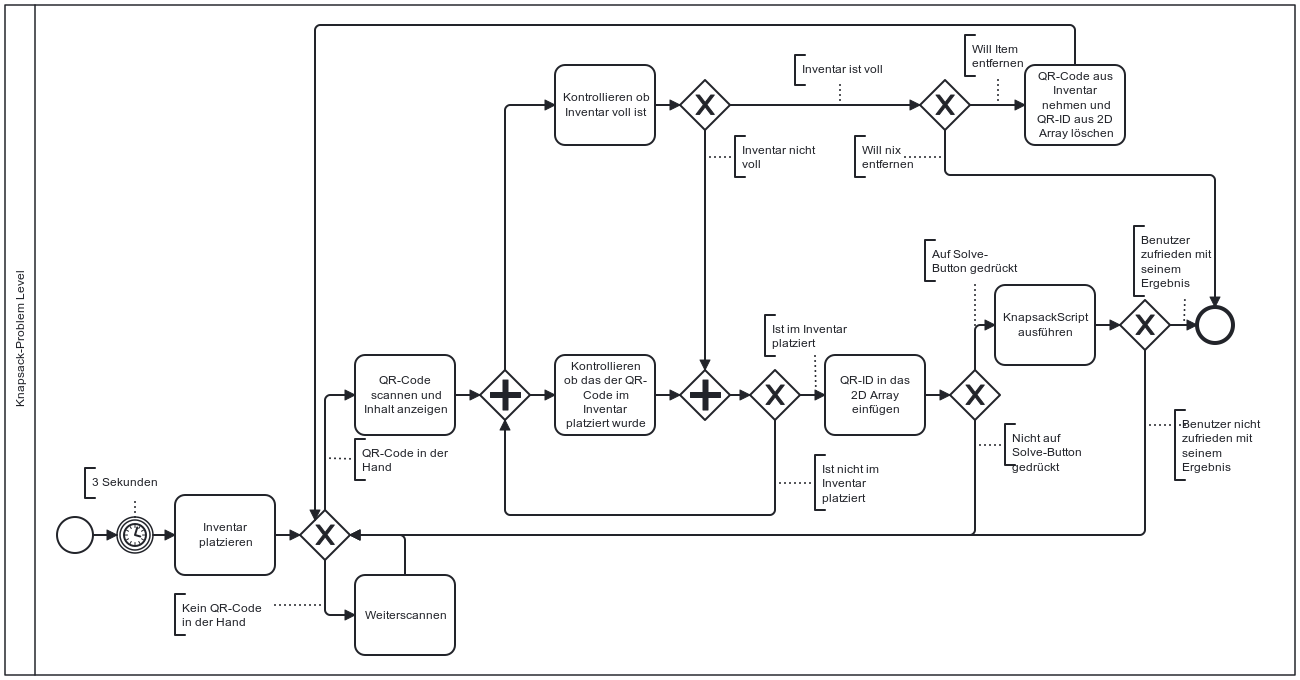
\includegraphics[scale=0.5, angle=270]{images/AblaufdiagrammLevel2}
    \caption{Ablaufdiagramm des Knapsack-Problem Levels}
    \label{fig:Ablaufdiagramm Level 2}
\end{figure}

\subsection{Mockups}
Hier steht der allgemeine Text für die Mockups

\section{Eingesetzte Technologien}

\subsection{Kriterien}
Bei der Auswahl der eingesetzten Technologien war es besonders wichtig, dass diese möglichst
zuverlässig und bereits etabliert sind. Die Technologien sollen ausfallsicher, leicht benutzbar
und vorallem eine performant Verwendung der Applikation sicherstellen.

\subsection{Game Engine: Konzeption und Funktion}
Eine Game Engine stellt eine hochentwickelte und modulare Entwicklungsumgebung dar, die speziell für die Konzeption,
Gestaltung und Implementierung von interaktiven digitalen Spielen entwickelt wurde. Als komplexe Softwarearchitektur
bildet sie das Grundgerüst für die Realisierung von Spieleprojekten, wobei sie eine Vielzahl von Funktionen und
Werkzeugen bereitstellt, um den Entwicklungsprozess zu erleichtern und zu optimieren.

Im Kern vereint eine Game Engine verschiedene Module, die für unterschiedliche Aspekte der Spieleentwicklung zuständig
sind. Dazu gehören unter anderem die Grafik-Engine, die Physik-Engine, die Audio-Engine sowie Mechanismen für
Kollisionserkennung, Animationen und Künstliche Intelligenz. Durch diese modulare Struktur ermöglicht die Game Engine
eine effiziente und ressourcenschonende Entwicklung, indem sie Entwickler von der tiefen Implementierung grundlegender
Funktionen entlastet.

Die Grafik-Engine ist dabei verantwortlich für die Darstellung visueller Elemente, von 2D-Grafiken bis hin zu
komplexen 3D-Welten. Sie bietet Mechanismen zur Berechnung von Lichteffekten, Schatten, Texturen und Animationen.
Die Physik-Engine simuliert realistische physikalische Interaktionen, um eine authentische Umgebungsgestaltung und
realitätsnahe Bewegungen der Spielelemente zu gewährleisten. Die Audio-Engine ermöglicht die Integration von Klängen
und Musik, um die Spielerfahrung zu vertiefen.

Ein entscheidendes Merkmal einer Game Engine ist auch die Integration von Programmiersprachen wie C++ oder C#, die es
Entwicklern erlauben, spezifische Spiellogik und Interaktionen zu implementieren. Dieser Aspekt ermöglicht die
Flexibilität und Anpassbarkeit der Engine an die individuellen Anforderungen eines Spieleprojekts.

In der Gesamtheit fungiert die Game Engine als zentrale Schaltstelle für die kreative Entfaltung von Entwicklerteams,
indem sie eine umfassende Plattform für das Design und die Umsetzung von Spieleideen bietet. Ihre Funktionen reichen
von der effizienten Ressourcenverwaltung bis hin zur Bereitstellung von Werkzeugen für das Testen, Debuggen und
Optimieren von Spielen.

Die Auswahl einer geeigneten Game Engine ist eine strategische Entscheidung und hängt von den spezifischen
Anforderungen eines Projekts ab. In diesem Kontext wurden die beiden führenden Game Engines, Unity und Unreal Engine,
evaluiert, wobei Unity aufgrund seiner Programmiersprache C#, dem einfachen Einstieg für Anfänger, der exzellenten
Dokumentation und der umfangreichen Tutorial-Ressourcen als präferierte Wahl für das vorliegende Projektteam hervorging.

\subsubsection{Game Engine Auswahl und Wechsel im Projektverlauf}
Zu Projektbeginn standen zwei der führenden Game Engines zur Auswahl – die Unreal Engine und Unity. Eine Game Engine
fungiert als komplexe Softwareumgebung, speziell entwickelt für das Design und die Entwicklung von digitalen Spielen.
Die Auswahl einer geeigneten Engine beeinflusst maßgeblich den Entwicklungsprozess und den Erfolg eines Projekts.

Nach einer gründlichen Recherche und Evaluierung der beiden Optionen entschied sich das Projektteam für Unity als
präferierte Game Engine. Diese Entscheidung wurde durch mehrere Schlüsselfaktoren gestützt:

\begin{itemize}
    \item \textbf{Programmiersprache: C#} - Die Verwendung der Programmiersprache C# erwies sich als entscheidend,
    da sie sich als äußerst effizient und benutzerfreundlich herausstellte.
    \item \textbf{Einfacher Einstieg für Anfänger} - Unity bietet einen leicht verständlichen Einstieg in die
    Spieleentwicklung, was besonders für Teammitglieder mit unterschiedlichem Erfahrungsniveau von Vorteil ist.
    \item \textbf{Sehr gute Dokumentation} - Die umfassende Dokumentation von Unity spielte eine zentrale Rolle für
    effiziente Entwicklung und Problemlösung im gesamten Projektverlauf.
    \item \textbf{Hohe Anzahl an Tutorials} - Unity überzeugte mit einer reichhaltigen Sammlung von Tutorials und
    Schulungsmaterialien, die eine kontinuierliche Weiterbildung und schnelle Lösung von Herausforderungen ermöglichten.
\end{itemize}

Ursprünglich war die Unreal Engine aufgrund ihres beliebten Blueprint-Scripting-Systems in Betracht gezogen worden.
Jedoch traten im Verlauf der Entwicklungsarbeit spezifische Herausforderungen auf, die zu einer strategischen
Entscheidung für den Wechsel zur Unity Game Engine führten. Die Herausforderungen umfassten:

\begin{enumerate}
    \item \textbf{Mangelhafte Dokumentation für AR-Entwicklung in der Unreal Engine:} Die unzureichende Dokumentation
    für die Entwicklung von Augmented Reality (AR)-Anwendungen in der Unreal Engine erwies sich als erhebliche Hürde.
    Fehlende detaillierte Anleitungen und Referenzen für AR-spezifische Funktionen behinderten die effiziente Integration von AR-Elementen.
    \item \textbf{Begrenzte Verfügbarkeit von AR-spezifischen Online-Tutorials:} Ein Mangel an Online-Tutorials,
    die sich speziell mit der Entwicklung von AR-Anwendungen in der Unreal Engine befassten, führte zu einer
    beträchtlichen Lernkurve für das Entwicklerteam und verzögerte den Implementierungsprozess von AR-spezifischen Features.
    \item \textbf{Komplexität der AR-Entwicklung in der Unreal Engine:} Die Unreal Engine erwies sich als
    anspruchsvoller in Bezug auf die Umsetzung von AR-spezifischen Funktionen. Die Notwendigkeit, komplexe Skripte zu
    erstellen und vielfältige Einstellungen anzupassen, führte zu einem erhöhten Zeitaufwand für die Umsetzung von AR-Elementen.
    \item \textbf{Mangelhafte Integration von AR-spezifischen Werkzeugen:} Schwächen in der Integration von
    AR-spezifischen Entwicklungswerkzeugen in der Unreal Engine erschwerten eine nahtlose Interaktion mit AR-Plattformen
    und die optimale Nutzung ihrer Funktionen.
    \item \textbf{Eingeschränkte Community-Unterstützung für AR-Entwicklung:} Im Vergleich zu Unity war die Community-Unterstützung
    für die AR-Entwicklung in der Unreal Engine begrenzt. Die Verfügbarkeit von Ratschlägen und Lösungen für spezifische
    AR-Herausforderungen war eingeschränkt, was die Eigenständigkeit bei der Lösung von Problemen beeinträchtigte.
\end{enumerate}

Diese Herausforderungen bildeten die Grundlage für die strategische Entscheidung des Projektteams, von der Unreal Engine
zu Unity zu wechseln. Der Wechsel ermöglichte eine effizientere und zielführende Entwicklung der AR-Applikation,
gestützt durch Unity's umfassende Unterstützung, detaillierte Dokumentation und breite Community-Ressourcen.


\subsection{Unity foundation packages}
%Quellen:
In dem folgenden Abscnhitt wird erklärt welche Packages in die Unity Applikation
eingeführt werden müssen um die Entwicklung einer Augmented Reality Applikation ohne Problem
ermöglichen zu können.

\subsubsection{MRTK3}
Das Mixed Reality Toolkit (MRTK) \footnote{Microsoft \cite{MRTK3}} ist eine Sammlung von Tools,
Skripten und Ressourcen, die speziell für die Entwicklung von Mixed-Reality-Anwendungen, einschließlich Augmented
Reality, in Unity entwickelt wurden. MRTK3 ist eine Weiterentwicklung der vorherigen Versionen und bietet viele
Vorteile für AR-Anwendungen:
\begin{itemize}
    \item Interaktions- und Benutzerführung: \\
    MRTK3 stellt eine Reihe von Interaktionskomponenten und -systemen zur
    Verfügung, die es Entwicklern ermöglichen, intuitivere Benutzererfahrungen in AR-Anwendungen zu gestalten.
    Dies umfasst Dinge wie das Platzieren von Objekten in der realen Welt, die Verfolgung von Handgesten und die
    Unterstützung von Blickverfolgung.
    \item Standardisierte APIs: \\
    Durch die Verwendung von MRTK3 kannst du auf standardisierte APIs und Komponenten
    zugreifen, die speziell für AR-Anwendungen entwickelt wurden. Dies erleichtert die Implementierung von Funktionen
    wie Handgesten, Sprachsteuerung und Objektplatzierung.
    \item Einfache Konfiguration und Anpassung: \\
    MRTK3 bietet eine einfache Konfiguration und Anpassung über die
    Unity-Oberfläche. Dies erleichtert die Anpassung deiner AR-Anwendung an spezifische Anforderungen und Use Cases.
\end{itemize}

\subsubsection{Microsoft OpenXR Plugin}
Das Microsoft OpenXR Plugin \footnote{Khronos \cite{OpenXR}} ist eine Sammlung von Tools ist ein wichtiges Plugin für Unity, das die Integration von OpenXR-Unterstützung in
die AR-Anwendung ermöglicht. OpenXR ist ein offener Industriestandard, der die Entwicklung von XR
(Extended Reality)-Anwendungen, einschließlich Augmented Reality, erleichtert. Anschließend ein paar Punkte wieso
dieses Plugin so wichtig ist:
\begin{itemize}
    \item Geräteunabhängigkeit: \\
    Durch die Verwendung von OpenXR und dem Microsoft OpenXR Plugin kann die AR-Anwendung auf verschiedenen
    XR-Geräten ausgeführt werden, ohne die Kernfunktionalität für jedes einzelne Gerät neu entwickeln zu müssen.
    Dies gewährleistet eine reibungslose Interaktion mit der HoloLens 2 und anderen XR-Geräten.
    \item Leistungssteigerung und Stabilität: \\
    Die Nutzung von OpenXR und des Microsoft OpenXR Plugins kann die
    Leistung und Stabilität der AR-Anwendung erheblich verbessern. Sie gewährleisten eine reibungslose Ausführung
    der Anwendung auf dem Zielsystem und bieten eine optimale Benutzererfahrung.
\end{itemize}

\subsection{Modellierungsprogramm}

Die Erstellung der 3D-Modelle für die beiden Level erfordert ein Rendering-Programm. Die Entscheidung für das
Rendering-Programm Blender wurde bereits zu Beginn des Projekts getroffen. \\
Diese Wahl basiert auf folgenden Gründen:
\begin{itemize}
    \item \textbf{Kostenfrei und Open Source}\\
    Blender ist kostenfrei und quelloffen, was bedeutet, dass es ohne Lizenzkosten genutzt werden kann. Dies ist
    besonders attraktiv bei der Entwicklung von AR-Anwendungen mit begrenztem Budget.
    \item \textbf{Echtzeit-Rendering}\\
    Blender verfügt über einen Echtzeit-Renderer namens Eevee, der schnelle Vorschauen
    und Renderings ermöglicht. Dies ist hilfreich, um AR-Inhalte in Echtzeit anzuzeigen und zu überprüfen.

    \item \textbf{Integration mit AR-Frameworks}\\
    Obwohl Blender keine direkte Unterstützung für AR-Funktionen bietet, können die erstellten 3D-Modelle und
    Animationen in AR-Entwicklungsumgebungen wie Unity oder Unreal Engine importiert werden, um dort
    AR-spezifische Funktionalitäten hinzuzufügen.
\end{itemize}

\subsubsection{Wie funktioniert Blender im Allgemeinen?}

Die nachfolgende Beschreibung hebt die Schlüsselaspekte und die Funktionalität von Blender für unseren speziellen
Anwendungsbereich hervor.

\begin{itemize}
    \item \textbf{Benutzeroberfläche und Interaktion}\\
    Die Benutzeroberfläche von Blender ist komplex gestaltet, aber hoch anpassbar. Sie enthält 3D-Modelle,
    Ansichten, Fenster und Panels. Benutzer interagieren mit Objekten und Werkzeugen über Maus- und Tastaturbefehle,
    wobei erfahrene Nutzer Hotkeys oder Shortcuts verwenden können, um effizienter zu arbeiten.

    \item \textbf{3D-Modellierung}\\
    Blender ermöglicht die Erstellung von 3D-Modellen durch die Verwendung von Primitiven wie Würfeln, Kugeln,
    Flächen und Kurven. Diese können dann bearbeitet und modifiziert werden, um komplexe Formen zu erstellen.
    Modellierungswerkzeuge umfassen Extrusion, Verschiebung, Skalierung und Rotation.

    \item \textbf{Materialien und Texturen}\\
    Zur Erzeugung realistischer Oberflächen können Materialien erstellt und Texturen auf Objekte angewendet werden.
    Blender erlaubt die Feinanpassung von Materialeigenschaften wie Diffusreflexion, Glanz, Transparenz und Emission.

    \item \textbf{Gemeinschaft und Ressourcen}\\
    Blender verfügt über eine engagierte Benutzergemeinschaft, die umfassende Dokumentation, Tutorials und Foren
    bereitstellt. Diese Ressourcen erleichtern die Einarbeitung und die Lösung von Problemen.

\end{itemize}
Blender kommt in unserer Diplomarbeit in beiden Leveln zum Einsatz. Die Hauptanwendung des Programms findet im Level 2
statt, wo Blender für die digitale Modellierung wichtiger täglicher Gegenstände von Schülern genutzt wird. Das Ziel ist
es, am Ende eine umfangreiche Sammlung von Objekten zu haben, um den Benutzern eine vielfältige Auswahl zu bieten.
